\chapter{Alberi binari di ricerca e alberi bilanciati}
\section{Alberi binari di ricerca}
Precedentemente abbiamo accennato al concetto di \hyperref[def:39]
{\emph{dizionario}}, ovvero una \emph{struttura dati} costituita da coppie
chiave-valore. Un \emph{dizionario} può essere implementato in molteplici modi e
come abbiamo visto, implementazioni diverse possono comportare \emph{complessità}
diverse per le singole operazioni che agiscono su quella \emph{struttura}.

Ad, esempio, la seguente tabella riporta le complessità delle operazioni per
tre possibili implementazioni:
\begin{table}[h]
    \renewcommand{\arraystretch}{1.2}
    \centering
    \begin{tabular}{|l|c|c|c|}
        \hline
        \textbf{Struttura dati} & \textbf{lookup} & \textbf{insert} & \textbf{remove}\\
        \hline
        Vettore ordinato & $O(\log n)$ & $O(1)$ & $O(n)$\\
        \hline
        Vettore non ordinato & $O(n)$ & $O(1)$ & $O(1)$\\
        \hline
        Lista non ordinata & $O(n)$ & $O(1)$ & $O(1)$\\
        \hline
    \end{tabular}
\end{table}

\begin{note}
    La \emph{complessità} delle operazioni di \texttt{insert} e \texttt{remove}
    per le implementazioni con \emph{vettore e lista non ordinati} è $O(1)$
    solo se si ipotizza che, nella \texttt{insert} non si debba verificare se
    l'elemento è già presente o meno, e nella \texttt{remove}, che si conosca
    già la posizione dell'elemento da rimuovere. Se non si fanno queste
    ipotesi, la \emph{complessità} diventa $O(n)$.
\end{note}\noindent
A questo punto ci chiediamo se non sia possibile implementare un \emph{dizionario}
sfruttando gli \emph{alberi binari}. Supponiamo che ogni \emph{nodo}
contenga una coppia formata da una chiave e un valore. E ipotizziamo anche che
le chiavi appartengano ad un insieme totalmente ordinato, cioè che sia sempre
possibile stabile se una chiave precede o meno un'altra.
L'implementazione di un \emph{nodo} dell'\emph{albero} potrebbe quindi essere:
\begin{code}{Nodo albero}
    \bc{TREE} parent\\
    \bc{TREE} left\\
    \bc{TREE} right\\
    \bc{ITEM} key, value
\end{code}\noindent
Poiché le chiavi sono ordinabili, possiamo ipotizzare che per ogni \emph{nodo}
$u$ valgano le seguenti due proprietà:
\begin{enumerate}
    \item Le chiavi contenute nel \emph{sottoalbero sinistro} di $u$ sono
    tutte minori di $u.key$;
    \item Le chiavi contenute nel \emph{sottoalbero destro} di $u$ sono
    tutte maggiori di $u.key$;
\end{enumerate}\newpage
\begin{note}
    Le proprietà appena definite permettono di realizzare un algoritmo di
    ricerca dicotomica.
\end{note}\noindent
Definiamo una regola generale:\
\begin{definition}[Albero binario di ricerca (ABR)]
    Un albero binario di ricerca è un albero binario nel quale per ogni nodo $u$
    vale:
    \begin{enumerate}
        \item Ogni nodo del sottoalbero sinistro ha un valore inferiore di quello
        del nodo $u$;
        \item Ogni nodo del sottoalbero destro ha un valore maggiore di quello
        del nodo $u$;
    \end{enumerate}
\end{definition}

\subsection{Specifica}
Per un \emph{dizionario} implementato come \emph{albero binario di ricerca}
possiamo definire la seguente \emph{specifica}.
\begin{code}{Dizionario come albero binario di ricerca}
    \com{Getter}
    \bc{TREE} parent()\\
    \bc{TREE} left()\\
    \bc{TREE} right()\\
    \bc{ITEM} key()\\
    \bc{ITEM} value()\\
    
    \noindent\com{Operazioni per il \emph{dizionario}}
    \bc{ITEM} lookup(\bc{ITEM} k)\\
    insert(\bc{ITEM} k, \bc{ITEM} v)\\
    remove(\bc{ITEM} k)\\
    
    \noindent\com{Operazioni definibili su un \emph{albero di ricerca binaria}}
    \nl\com{Restituisce il nodo successore di $t$, cioè il più piccolo}
    \com{tra i \emph{nodi} più grandi di $t$}
    \bc{TREE} successorNode(\bc{TREE} t)
    \nl\com{Restituisce il nodo predecessore di $t$, cioè il più grande}
    \com{tra i \emph{nodi} più piccoli di $t$}
    \bc{TREE} predecessorNode(\bc{TREE} t)
    \nl\com{Restituisce il \emph{nodo} con valore minore}
    \bc{TREE} min(\bc{TREE} t)
    \nl\com{Restituisce il \emph{nodo} con valore maggiore}
    \bc{TREE} max(\bc{TREE} t)\\

    \noindent\com{Funzioni interne ausiliarie}
    \nl\com{Restituisce il \emph{nodo} dell'\emph{albero} $t$ contenente la
    chiave $k$,}
    \com{se è presente, altrimenti nil}
    \bc{TREE} lookupNode(\bc{TREE} t, \bc{ITEM} k)
    \nl\com{Inserisce l'associazione chiave-valore $(k, v)$ nell'\emph{albero} $t$.}
    \com{Se la chiave è già presente sostituisce il valore associato, altrimenti}
    \com{viene inserita una nuova associazione.}
    \com{Se $t$ è nil restituisce il \emph{nodo} creato, altrimenti $t$}
    \bc{TREE} insertNode(\bc{TREE} t, \bc{ITEM} k, \bc{ITEM} v)
    \nl\com{Rimuove il \emph{nodo} associato alla chiave $k$ e restituisce la
    \emph{radice}}
    \com{dell'\emph{albero} (potrebbe essere stata cambiata)}
    \bc{TREE} removeNode(\bc{TREE} t, \bc{ITEM} k)
\end{code}

\paragraph{Implementazione dizionario}
Operazioni a parte, l'implementazione di \emph{dizionario} mediante \emph{albero
binario di ricerca} non è altro che:
\begin{code}{Dizionario come ABR}
    \bc{TREE} tree\\

    \ind Dictionary()\\
        tree = nil
\end{code}

\subsection{Ricerca}
L'implementazione della funzione \texttt{lookup} è banale:
\begin{minicode}{Dizionario come ABR - lookup}
    \ind\bc{ITEM} lookup(\bc{ITEM} k)\\
    \bc{TREE} t = lookupNode(tree, k)\\
    \indf if (t $\neq$ nil) then\\
        return t.value()\\
    \indf else\\
        return nil
\end{minicode}\noindent
La \texttt{lookupNode} può essere implementata sia in modo ricorsivo che
iterativo:
\begin{code}{Implementazione ricorsiva e iterativa di lookupNode}
    \begin{minipage}[t]{0.50\textwidth}
        \com{Versione ricorsiva}
        \rmbreak\ind\bc{TREE} lookupNode(\bc{TREE} t, \bc{ITEM} k)\\
            \indf if (t == nil or t.key == k) then\\
                return t\\
            \indf else\\
                \indff if (k < t.key) then\\
                    return lookupNode(t.left, k)\\
                \indff else\\
                    return lookupNode(t.right, k)\\
    \end{minipage}
    \hfill
    \begin{minipage}[t]{0.48\textwidth}
        \com{Versione iterativa}
        \rmbreak\ind\bc{TREE} lookupNode(\bc{TREE} t, \bc{ITEM} k)\\
            \bc{TREE} u = t\\
            \indf while (t $\neq$ nil and t.key $\neq$ k) do\\
                \indff if (k < u.key) then\\
                    \com{Sottoalbero di sinistra}
                    u = u.left\\
                \indff else\\
                    \com{Sottoalbero di destra}
                    u = u.right\\
            \indf return u
    \end{minipage}
\end{code}

\subsection{Massimo e minimo}
Grazie alle proprietà degli \emph{alberi binari di ricerca} la ricerca del
minimo e del massimo si riduce alla ricerca del \emph{nodo} più a sinistra
e più a destra dell'\emph{albero}.

\begin{code}{Implementazione minimo e massimo}
    \begin{minipage}[t]{0.48\textwidth}
        \com{Ricerca del minimo}
        \rmbreak\ind\bc{TREE} min(TREE t)\\
            \bc{TREE} u = t\\
            \indf if (u == nil) do\\
                return u\\
            \indf while (u.left $\neq$ nil) do\\
                u = u.left\\
            \indf return u
    \end{minipage}
    \hfill
    \begin{minipage}[t]{0.48\textwidth}
        \com{Ricerca del massimo}
        \rmbreak\ind\bc{TREE} max(TREE t)\\
            \bc{TREE} u = t\\
            \indf if (u == nil) do\\
                return u\\
            \indf while (u.right $\neq$ nil) do\\
                u = u.right\\
            \indf return u
    \end{minipage}
\end{code}

\subsection{Successore e predecessore}
\begin{definition}[Successore]
    Il successore di un nodo $u$ è il più piccolo nodo maggiore di $u$.
\end{definition}
\begin{definition}[Predecessore]
    Il predecessore di un nodo $u$ è il più grande nodo minore di $u$.
\end{definition}

\paragraph{Ricerca del successore}
Poiché il \emph{successore} di un \emph{nodo} è il più piccolo tra i \emph{nodi}
maggiori di esso, la ricerca del \emph{successore} di un \emph{nodo} $u$ non
può che essere fatta sui \emph{nodi} maggiori di $u$.
A questo punto quindi, si configurano due casi:
\begin{enumerate}
    \item \emph{$u$ ha un figlio destro}: il \emph{successore} di $u$ è
    il \emph{minimo} tra i \emph{nodi} del suo \emph{sottoalbero destro};
    \item \emph{$u$ non ha un figlio destro}: il \emph{successore}, se esiste, è
    uno degli \emph{avi} di $u$, ovvero uno dei \emph{nodi} superiori.
    Quindi, risalendo l'\emph{albero}, il \emph{successore} è il primo \emph{nodo}
    maggiore di $u$, cioè il primo \emph{nodo} per il quale $u$ sta nel suo
    \emph{sottoalbero sinistro};
\end{enumerate}

\begin{minicode}{Implementazione successore}
    \ind\bc{TREE} successorNode(\bc{TREE} t)\\
        \indf if (t == nil) then
            return t\\
        \indf if (t.right $\neq$ nil)\hfill\com{Caso 1:\,$t$ ha un \emph{figlio destro}}
            return min(t.right)\\
        \indf else\hfill\com{Caso 2:\,$t$ non ha un \emph{figlio destro}}
            \bc{TREE} p = t.parent\\
            \indff while (p $\neq$ nil and t == p.right) do\\
                t = p\\
                p = p.parent\\
            \indff return p
\end{minicode}

\paragraph{Ricerca del predecessore}
Per il \emph{predecessore} valgono le stesse considerazioni fatte per la
ricerca del \emph{successore}, ad eccezione del fatto che, se esiste, il
\emph{predecessore} di un \emph{nodo} $u$ sarà il massimo del suo \emph{sottoalbero
sinistro} oppure il primo \emph{avo} che ha $u$ come elemento del
\emph{sottoalbero destro}.

\begin{minicode}{Implementazione predecessore}
    \ind\bc{TREE} successorNode(\bc{TREE} t)\\
        \indf if (t == nil) then
            return t\\
        \indf if (t.left $\neq$ nil)\hfill\com{Caso 1:\,$t$ ha un \emph{figlio sinistro}}
            return max(t.left)\\
        \indf else\hfill\com{Caso 2:\,$t$ non ha un \emph{figlio sinistro}}
            \bc{TREE} p = t.parent\\
            \indff while (p $\neq$ nil and t == p.left) do\\
                t = p\\
                p = p.parent\\
            \indff return p
\end{minicode}

\subsection{Inserimento}
Per eseguire l'inserimento di una nuova associazione nel \emph{dizionario} è
sufficiente fare uso della funzione \texttt{insertNode}, che va ad inserire un
\emph{nodo}, o a modificarne uno esistente, in un \emph{albero binario di
ricerca}.
\begin{minicode}{Dizionario come ABR - insert}
    \ind insert(\bc{ITEM} k, \bc{ITEM} v)\\
        \indf tree = insertNode(tree, k, v)\\
\end{minicode}\noindent
Nemmeno l'implementazione della \texttt{insertNode} crea molti problemi, in quanto
è sufficiente applicare ricorsivamente le \hyperref[def:44]{\emph{proprietà degli
alberi binari di ricerca}}. Andremo quindi ad invocare ricorsivamente
l'\texttt{insertNode}, sul \emph{sottoalbero sinistro} o \emph{destro} a seconda
della relazione d'ordine tra il valore del nodo (i.e il valore della chiave
associata al \emph{nodo}) e il valore della chiave da inserire, fino al
raggiungimento di una \emph{foglia}, alla quale aggiungeremo un nuovo \emph{figlio
destro} o \emph{sinistro}, o di un \emph{nodo}, associato ad una chiave con lo
stesso valore di quella da inserire, nel qual caso sostituiremo il valore
salvato nel \emph{nodo} con quello nuovo.

Prima però di passare all'implementazione vera e propria, definiamo una
funzione ausiliaria \texttt{link} che presi due \emph{nodi} $p$, $u$ e una
chiave $k$, inserisce il \emph{nodo} $u$ come \emph{figlio sinistro} di $p$ se
$p.key > k$, altrimenti lo inserisce come \emph{figlio destro}.

\begin{minicode}{Implementazione link}
    \ind link(\bc{TREE} p, \bc{TREE} u, \bc{ITEM} k)\\
        \indf if (u $\neq$ nil) then\\
            u.parent = p\hfill\com{Inserisce il riferimento al \emph{padre}}
        \indf if (p $\neq$ nil) then\\
            \indff if (p.key > k) then\\
                p.left = u\hfill\com{Inserisce $u$ come \emph{figlio sinistro}}
            \indff else\\
                p.right = u\hfill\com{Inserisce $u$ come \emph{figlio destro}}
\end{minicode}

\begin{minicode}{Implementazione ricorsiva insertNode}
   \ind\bc{TREE} insertNode(\bc{TREE} t, \bc{ITEM} k, \bc{ITEM} v)\\
        \com{L'\emph{albero} è vuoto, quindi creo un nuovo \emph{nodo} e lo restituisco}
        \indf if (t == nil) then\\
            return Tree(k, v)\\
        \indf if (t.key == k) then\\
            t.value = v\hfill\com{L'associazione esiste già, per cui aggiorno il valore}
            return t\\
        \indf if (t.key > k) then\\
            \indff if (t.left == nil) then\hfill\com{Inserisce il \emph{nodo} come \emph{figlio sinistro}}
                link(t, Tree(k, v), k)\\
                return t\\
            \indff else\\
                return insertNode(t.left, k, v)\hfill\com{Continua a discendere l'\emph{albero}}
        \indf else\\
            \indff if (t.right == nil) then\hfill\com{Inserisce il \emph{nodo} come \emph{figlio destro}}
                link(t, Tree(k, v), k)\\
                return t\\
            \indff else\\
                return insertNode(t.right, k, v)\hfill\com{Continua a discendere l'\emph{albero}}
\end{minicode}\noindent
È anche possibile realizzare una versione iterativa della \texttt{insertNode}

\begin{minicode}{Implementazione iterativa insertNode}
\ind\bc{TREE} insertNode(\bc{TREE} t, \bc{ITEM} k, \bc{ITEM} v)\hfill\com{Riferimento al \emph{padre}}
    \bc{TREE} p = nil\\
    \bc{TREE} u = t\\
    \indf while (u $\neq$ nil and u.key $\neq$ k) do\hfill\com{Cerca la posizione di inserimento}
        p = u\\
        u = iif(k < u.key, u.left, u.right)\\
    \indf if (u $\neq$ nil and u.key == k) then\hfill\com{La chiave è già presente}
        u.value = v\\
    \indf else\\
        \bc{TREE} newTree = Tree(k, v)\hfill\com{Crea un nuovo \emph{nodo}}
        link(p, newTree, k)\hfill\com{Inserisce il nuovo \emph{nodo}}
        \indff if (p == nil) then\hfill\com{Il \emph{nodo creato è il primo dell'\emph{albero}}}
            t = newTree\\
    \indf return t\hfill\com{Restituisce il nuovo \emph{albero} o quello modificato}
\end{minicode}

\subsection{Cancellazione}
Come per la ricerca e l'inserimento, anche l'implementazione della funzione
\texttt{remove} è basata su un'altra funzione, la \texttt{removeNode}.

\begin{minicode}{Dizionario come ABR - remove}
    \ind remove(\bc{ITEM} k)\\
        tree = removeNode(tree, k)
\end{minicode}\noindent
L'implementazione della \texttt{removeNode} non è per nulla banale, in quanto, se
$u$ è il \emph{nodo} da eliminare, vanno considerate diverse casistiche:
\begin{enumerate}
    \item \emph{$u$ non ha figli}: si elimina il \emph{nodo};
    \item \emph{$u$ ha un figlio $f$}: si elimina $u$ e si rende $f$ il \emph{figlio}
    dell'\emph{ex-padre} di $u$ in sostituzione di $u$ (\emph{short-cut});
    \item \emph{$u$ ha due figli}: si individua il \emph{successore} $s$ di $u$.
    Poiché il \emph{successore}, per definizione, non ha \emph{figlio sinistro},
    si stacca $s$ dal proprio \emph{padre} e si attacca il suo \emph{figlio
    destro}, se esiste, come \emph{figlio sinistro} del \emph{padre} di $s$.
    Infine, si copia il valore di $s$ su $u$ e si elimina $s$;
\end{enumerate}

\begin{minicode}{Implementazione removeNode}
\ind\bc{TREE} removeNode(\bc{TREE} t, \bc{ITEM} k)\\
    \bc{TREE} u = lookupNode(t, k)\\
    \indf if (u $\neq$ nil) then\\
        \indff if (u.left == nil and u.right == nil) then\hfill\com{Caso 1}
            link(u.parent, nil, k)\hfill\com{Rimuove il \emph{figlio}}
            delete u\\
        \indff else if (u.left $\neq$ nil and u.right $\neq$ nil) then\hfill\com{Caso 3}
            \bc{TREE} s = successorNode(u)\\
            link(s.parent, s.right, s.key)\hfill\com{Attacca il \emph{figlio} di $s$ al \emph{padre} di $s$}
            u.key = s.key\hfill\com{Copia su $u$ la chiave di $s$}
            u.value = s.value\hfill\com{Copia su $u$ il valore di $s$}
            delete s\\
        \indff else if (u.left $\neq$ nil and u.right == nil)\hfill\com{Caso 2 con \emph{figlio sinistro}}
            link(u.parent, u.left, k)\\
            \indfff if (u.parent == nil) then\\
                t = u.left\\
        \indff else\hfill\com{Caso 2 con \emph{figlio destro}}
            link(u.parent, u.right, k)\\
            \indfff if (u.parent == nil) then\\
                t = u.right\\
    \indf return t
\end{minicode}\noindent
Vediamo la dimostrazione della correttezza di questa implementazione:
\begin{proof}[Dimostrazione]
    Procediamo caso per caso. Sia $u$ il \emph{nodo} che si
    intende rimuovere dall'\emph{albero}:
    \begin{enumerate}
        \item \emph{Nessun figlio}: eliminare \emph{foglie} non inficia
        sull'ordine degli altri nodi;
        \item \emph{Un solo figlio}:
        \begin{enumerate}
            \item \emph{Figlio destro}: se $u$ è il \emph{figlio destro} di $p$
            tutti i valori nell'\emph{albero} che ha come \emph{radice} $u$ sono
            maggiori di $p$;
            \item \emph{Figlio sinistro}: se $u$ è il \emph{figlio sinistro} di $p$
            tutti i valori nell'\emph{albero} che ha come \emph{radice} $u$ sono
            minori di $p$;
        \end{enumerate}
        \item \emph{Due figli}: il \emph{successore} $s$ del \emph{nodo} è
        maggiore di tutti i nodi del \emph{sottoalbero di sinistra} di $u$,
        ma allo stesso tempo, è anche minore di tutti i \emph{nodi} nel
        \emph{sottoalbero destro} di $u$, di conseguenza può essere sostituito
        a $u$;
    \end{enumerate}
\end{proof}

\subsection{Costo computazionale delle operazioni}
Tutte le operazioni viste per gli \emph{alberi binari di ricerca} sono
confinate ai \emph{nodi} posizionati lungo un cammino semplice dalla
\emph{radice} a una \emph{foglia}. Di conseguenza, se $h$ è l'\emph{altezza}
di un \emph{albero}, tutte le operazioni sono $O(h)$.

A questo punto vale la pena chiedersi quali siano il caso peggiore e quello
migliore.

\begin{figure}[h!]
    \centering
    \subfloat[Caso peggiore $h=O(n)$]
    {
        \begin{graph}
            \node[main, scale=0.8] (0) {$4$};
            \node[main, scale=0.8] (1) [below right of=0, xshift=-15] {$6$};
            \node[main, scale=0.8] (2) [below right of=1, xshift=-15] {$8$};
            \node[main, scale=0.8] (3) [below right of=2, xshift=-15] {$10$};
            \node[main, scale=0.8] (4) [below right of=3, xshift=-15] {$12$};
            \node[main, scale=0.8] (5) [below right of=4, xshift=-15] {$15$};
            \node[main, scale=0.8] (6) [below right of=5, xshift=-15] {$18$};
        
            \path[-]    (0) edge (1)
                        (1) edge (2)
                        (2) edge (3)
                        (3) edge (4)
                        (4) edge (5)
                        (5) edge (6);
        \end{graph}
    }
    \hspace{3cm}
    \subfloat[Caso migliore $h=O(\log n)$]
    {
        \begin{graph}
            \node[main] (0) [yshift=-107.5] {$10$};
            \node[main] (1) [below left of=0, xshift=-15] {$6$};
            \node[main] (2) [below right of=0, xshift=15] {$15$};
            \node[main] (3) [below left of=1, xshift=10] {$4$};
            \node[main] (4) [below right of=1, xshift=-10] {$8$};
            \node[main] (5) [below left of=2, xshift=10] {$12$};
            \node[main] (6) [below right of=2, xshift=-10] {$18$};
        
            \path[-]    (0) edge (1)
                        (0) edge (2)
                        (1) edge (3)
                        (1) edge (4)
                        (2) edge (5)
                        (2) edge (6);
        \end{graph}
    }
    \caption{\emph{Caso peggiore} e \emph{caso migliore}}
\end{figure}\noindent
Da queste immagini risulta evidente che sia meglio evitare di lavorare con \emph{alberi}
troppo \q{\emph{sbilanciati}}.

\section{Alberi binari di ricerca bilanciati}
Abbiamo terminato l'ultima sezione discutendo brevemente il modo in cui
l'\emph{altezza} di un \emph{albero} determini il costo delle operazioni. In
particolare, abbiamo accennato al fatto che nel caso pessimo tutti i \emph{nodi}
sono posizionati come in una \emph{lista}, mentre nel caso migliore
l'\emph{albero} gode una struttura più simmetrica rispetto alla \emph{radice}.

Ovviamente, nella maggior parte delle situazioni non si avrà a che fare né con
l'uno che con l'altro ed è quindi ragionevole attendersi, generalmente,
un'altezza inferiore a quella del caso pessimo. Addirittura, è dimostrato che
se gli elementi vengono inseriti in ordine casuale, l'\emph{altezza media} è
$O(\log n)$.

Nella realtà però, difficilmente ci si affida alla casualità e quindi, per
lavorare con \emph{alberi} di \emph{altezza} ottimale, si deve ricorrere a
tecniche che garantiscano un buon livello di \emph{bilanciamento}.

\begin{definition}[Fattore di bilanciamento]
    È definito fattore di bilanciamento di un nodo $v$ la massima differenza
    di l'altezza tra i suoi sottoalberi ed è indicato in simboli come $\beta(v)$.
\end{definition}\noindent
Esistono diversi algoritmi di \emph{bilanciamento}, quali ad esempio:
\begin{itemize}
    \item \emph{Alberi AVL} (Adelson-Veskii e Landis): bilanciano l'\emph{albero}
    facendo uso di rotazioni e garantiscono che per ogni \emph{nodo} $v$
    $\beta(v)\leq1$;
    \item \emph{B-alberi} (Bayer e McCreight): ogni \emph{nodo} $v$ ha
    $\beta(v)=0$ e sono specializzati per \emph{strutture} salvate in memoria
    secondaria;
    \item \emph{Alberi 2-3} (Hopcroft): ogni \emph{nodo} $v$ ha $\beta(v)=0$ e
    sono basati su una \emph{struttura} dinamica che attraverso operazioni di
    merge e split, distribuisce i \emph{nodi} su \emph{alberi} con due o tre
    \emph{figli};
\end{itemize}
In questa trattazione analizzeremo un quarto tipo di \emph{alberi}, gli
\emph{Alberi Red-Black}, ideati da Guibas e Sedgewick nel 1978.

\section{Alberi Red-Black}
\begin{definition}[Alberi Red-Black]
    Gli Alberi Red-Black sono alberi binari di ricerca nei quali ogni nodo è
    colorato di rosso oppure di nero. Le chiavi vengono mantenute soltanto nei
    nodi interni e le foglie sono costituite da nodi speciali con valore Nil.
    Inoltre, vengono rispettati i seguenti vincoli:
    \begin{enumerate}
        \item La radice è nera;
        \item Tutte le foglie sono nere;
        \item Entrambi i figli di un nodo rosso sono neri;
        \item Ogni cammino semplice da un nodo ad una delle sue foglie ha sempre
        lo stesso numero di nodi neri;
    \end{enumerate}
\end{definition}

\begin{figure}[h!]
    \centering
    \resizebox*{\textwidth}{!}{
        \begin{graph}
            \tikzset{rb/.style={main, font=\large\boldmath}}
            \tikzset{b/.style={rb, fill=black, color=black, text=red}}
            \tikzset{r/.style={rb, fill=red, color=red, text=black}}
            \tikzset{nil/.style={rectangle, fill=black, color=black, text=red, font=\ttfamily\large}}
        
            \node[b] (0) {$30$};
            \node[b] (1) [below left of=0, xshift=-100] {$15$};
            \node[b] (2) [below right of=0, xshift=100] {$70$};
        
            \node[b] (3) [below left of=1, xshift=-30] {$10$};
            \node[b] (4) [below right of=1, xshift=30] {$20$};
            \node[r] (5) [below left of=2, xshift=-30] {$60$};
            \node[b] (6) [below right of=2, xshift=30] {$85$};
        
            \node[r] (7) [below left of=3, xshift=7] {$5$};
            \node[b] (8) [below left of=5, xshift=7] {$50$};
            \node[b] (9) [below right of=5, xshift=-7] {$65$};
            \node[r] (10) [below left of=6, xshift=7] {$80$};
            \node[r] (11) [below right of=6, xshift=-7] {$90$};
        
            \node[r] (12) [below left of=8, xshift=24] {$40$};
            \node[r] (13) [below right of=8, xshift=-24] {$55$};
        
            \node[nil] (14) [below right of=3, xshift=-7] {Nil};
            \node[nil] (15) [below left of=4, xshift=7] {Nil};
            \node[nil] (16) [below right of=4, xshift=-7] {Nil};
        
            \node[nil] (23) [below left of=9, xshift=25, yshift=-5] {Nil};
            \node[nil] (24) [below right of=9, xshift=-25, yshift=-5] {Nil};
            \node[nil] (25) [below left of=10, xshift=25, yshift=-5] {Nil};
            \node[nil] (26) [below right of=10, xshift=-25, yshift=-5] {Nil};
            \node[nil] (27) [below left of=11, xshift=25, yshift=-5] {Nil};
            \node[nil] (28) [below right of=11, xshift=-25, yshift=-5] {Nil};
            \node[nil] (29) [below left of=7, xshift=25, yshift=-5] {Nil};
            \node[nil] (30) [below right of=7, xshift=-25, yshift=-5] {Nil};
        
            \node[nil] (31) [below left of=12, xshift=0] {Nil};
            \node[nil] (32) [below of=12, xshift=-3, yshift=16.5] {Nil};
            \node[nil] (33) [below of=13, xshift=3, yshift=16.5] {Nil};
            \node[nil] (34) [below right of=13, xshift=0] {Nil};
        
            \path[-]  (0) edge (1)
                      (0) edge (2)
                      (1) edge (3)
                      (1) edge (4)
                      (2) edge (5)
                      (2) edge (6)
                      (3) edge (7)
                      (5) edge (8)
                      (5) edge (9)
                      (6) edge (10)
                      (6) edge (11)
                      (8) edge (12)
                      (8) edge (13);
        
            \path[-]  (3) edge (14)
                      (4) edge (15)
                      (4) edge (16)
                      (9) edge (23)
                      (9) edge (24)
                      (10) edge (25)
                      (10) edge (26)
                      (11) edge (27)
                      (11) edge (28)
                      (7) edge (29)
                      (7) edge (30)
                      (12) edge (31)
                      (12) edge (32)
                      (13) edge (33)
                      (13) edge (34);
        \end{graph}
    }
    \caption{\emph{Albero Red-Black}}
    \label{fig:albero-red-black}
\end{figure}\noindent
Diamo inoltre le seguenti definizioni:
\begin{definition}[Altezza nera di un nodo]
    Dato un nodo $v$, l'altezza nera di quel nodo, indicata come $bh(v)$, è il
    numero di nodi neri lungo ogni cammino da $v$ (escluso) ad ogni sua foglia
    (inclusa).
\end{definition}
\begin{definition}[Altezza nera di un Albero Red-Black]
    L'altezza nera di un Albero Red-Black corrisponde all'altezza nera della
    sua radice.
\end{definition}\noindent
L'\emph{albero} della figura \ref{fig:albero-red-black} ha \emph{altezza nera}
pari a 3.

\begin{note}
    Per ogni \emph{Albero Red-Black} sono possibili più colorazioni che
    possono anche portare ad \emph{altezze nere} diverse.
\end{note}

\paragraph{Foglie come nodi Nil}
Come detto, le \emph{foglie} sono rappresentate da speciali \emph{nodi} con
valore \texttt{Nil}. Questo significa, che invece di un puntatore \texttt{nil},
c'è un riferimento ad un \emph{nodo} \texttt{Nil} di colore nero. E, poiché
tutti i \emph{nodi} \texttt{Nil} sono uguali, ne esiste uno solo al quale fanno
riferimento tutti i \emph{nodi} che hanno delle \emph{foglie}.

In realtà, i \emph{nodi} che hanno come \emph{figli} questo tipo di \emph{nodi},
sono essi stessi le vere foglie dell'\emph{albero}, in quanto, i \emph{nodi}
\texttt{Nil} non sono altro che \emph{sentinelle} create per permettere di
accedere al colore dei \emph{figli} senza dover gestire il caso in cui questi
siano \texttt{nil}.

\paragraph{Definizione di un nodo in un Albero Red-Black}
In generale, la definizione dei \emph{nodi} per \emph{Alberi Red-Black} non è
diversa da quella dei \emph{nodi} per \emph{alberi binari di ricerca} classici.
L'unica differenza sta nella necessità di tenere traccia del colore assegnato ad
ogni \emph{nodo}.

\begin{code}{Implementazione di un nodo in un Albero Red-Black}
    \bc{TREE} parent\\
    \bc{TREE} left\\
    \bc{TREE} right\\
    \bc{int} color\hfill\com{Per efficienza si sarebbe potuto usare un \bc{boolean}}
    \bc{ITEM} key, value
\end{code}

\subsection{Rotazioni}
Ogni volta che si va ad inserire un elemento in un \emph{Albero Red-Black} è
possibile che le \emph{condizioni di bilanciamento} vengano violate.

Quando ciò accade è possibile agire applicando delle operazioni di
\emph{rotazione}, oppure andando direttamente a modificare i colori dei \emph{nodi}
presenti nella zona in cui i vincoli risultano violati.

Una \emph{rotazione} prevede che la \emph{radice} di un \emph{albero} venga
sostituita con uno dei suoi \emph{figli}. Un'operazione di questo tipo, se
opportunamente sfruttata, permette di bilanciare un \q{\emph{albero sbilanciato}}.

\begin{figure}[h!]
\centering
\begin{tabular}[t]{c@{\quad}|@{\quad}c}
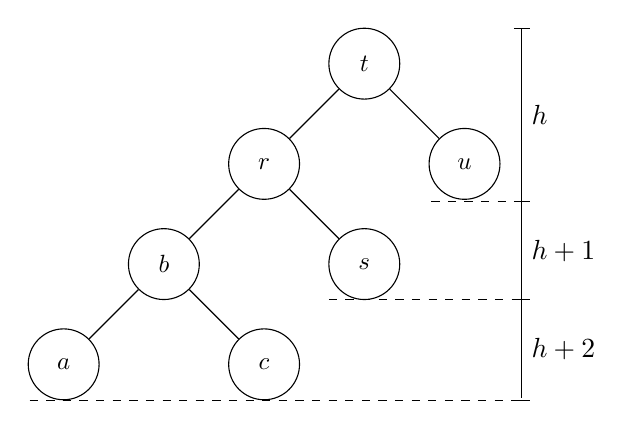
\begin{tikzpicture}[baseline={(0,0)},node distance={20mm},main/.style={draw, circle, scale=0.9, minimum size=10mm}]
    \node[main] (0) {$t$};

    \node[main] (1) [below left of=0] {$r$};
    \node[main] (2) [below right of=0] {$u$};

    \node[main] (3) [below left of=1] {$b$};
    \node[main] (4) [below right of=1] {$s$};

    \node[main] (5) [below left of=3] {$a$};
    \node[main] (6) [below right of=3] {$c$};

    \draw (0) -- (1);
    \draw (0) -- (2);
    \draw (1) -- (3);
    \draw (1) -- (4);
    \draw (3) -- (5);
    \draw (3) -- (6);

    \draw (2,0.45) -- (2,-1.75) node[midway, right] {$h$};
    \draw (1.9,0.45) -- (2.1,0.45);
    \draw [dashed] (0.85,-1.75) -- (1.9,-1.75);
    \draw (1.9,-1.75) -- (2.1,-1.75);
    \draw (2,-1.75) -- (2,-3) node[midway, right] {$h+1$};
    \draw [dashed] (-0.45,-3) -- (1.9,-3);
    \draw (1.9,-3) -- (2.1,-3);
    \draw (2,-3) -- (2,-4.25) node[midway, right] {$h+2$};
    \draw [dashed] (-4.25,-4.275) -- (1.9,-4.275);
    \draw (1.9,-4.275) -- (2.1, -4.275);
\end{tikzpicture} &
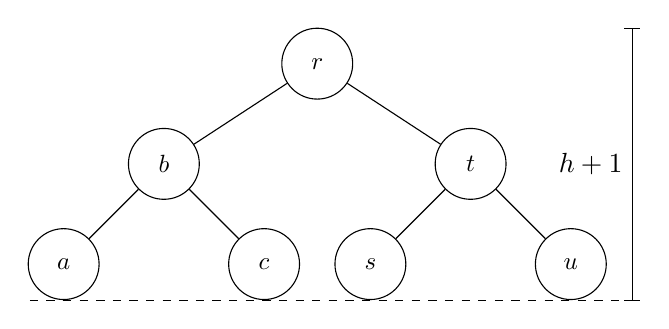
\begin{tikzpicture}[baseline={(0,0)},node distance={20mm},main/.style={draw, circle, scale=0.9, minimum size=10mm}]
    \node[main] (1) [] {$r$};

    \node[main] (0) [below right of=1, xshift=7.5mm] {$t$};
    \node[main] (2) [below right of=0] {$u$};

    \node[main] (3) [below left of=1, xshift=-7.5mm] {$b$};
    \node[main] (4) [below left of=0] {$s$};

    \node[main] (5) [below left of=3] {$a$};
    \node[main] (6) [below right of=3] {$c$};

    \draw (0) -- (1);
    \draw (0) -- (2);
    \draw (1) -- (3);
    \draw (0) -- (4);
    \draw (3) -- (5);
    \draw (3) -- (6);

    \draw (4,0.45) -- (4,-3) node[midway, left] {$h+1$};
    \draw (3.9,0.45) -- (4.1,0.45);
    \draw [dashed] (-3.65,-3.01) -- (3.9,-3.01);
    \draw (3.9,-3.01) -- (4.1,-3.01);
\end{tikzpicture}
\end{tabular}
\caption{Esempio di \emph{rotazione verso destra} del \emph{nodo} $t$}
\end{figure}

\begin{code}{Implementazione funzioni di rotazione}
\begin{minipage}[t]{0.48\textwidth}
    \com{Rotazione verso sinistra}
    \rmbreak\ind\bc{TREE} rotateLeft(\bc{TREE} r)\\
        \bc{TREE} s = r.right\\
        \bc{TREE} t = r.parent\\
        \nl\rmbreak\ind\\
        \com{Il \emph{sottoalbero sinistro} di $s$}
        \com{diventa il \emph{figlio destro} di $r$}
        r.right = s.left\\
        \indf if (s.left $\neq$ nil) then\\
            s.left.parent = r\\
        \nl\rmbreak\ind\\
        \com{$r$ diventa il \emph{figlio sinistro}}
        \com{di $s$}
        s.left = r\\
        r.parent = s\\

        \nl\rmbreak\ind\\
        \com{$s$ diventa il \emph{figlio} di $t$}
        s.parent = t\\
        \indf if (t $\neq$ nil) then\\
            \indff if (t.left == r) then\\
                t.left = s\\
            \indff else\\
                t.right = s\\
        \indf return s\\
\end{minipage}
\hfill
\begin{minipage}[t]{0.48\textwidth}
    \com{Rotazione verso destra}
    \rmbreak\ind\bc{TREE} rotateRight(\bc{TREE} r)\\
        \bc{TREE} b = r.left\\
        \bc{TREE} t = r.parent\\
        \nl\rmbreak\ind\\
        \com{Il \emph{sottoalbero destro} di $b$}
        \com{diventa il \emph{figlio sinistro} di $r$}
        r.left = b.right\\
        \indf if (b.right $\neq$ nil) then\\
            b.right.parent = r\\
        \nl\rmbreak\ind\\
        \com{$r$ diventa il \emph{figlio destro}}
        \com{di $b$}
        b.right = r\\
        r.parent = b\\

        \nl\rmbreak\ind\\
        \com{$b$ diventa il \emph{figlio} di $t$}
        b.parent = t\\
        \indf if (t $\neq$ nil) then\\
            \indff if (t.left == r) then\\
                t.left = b\\
            \indff else\\
                t.right = b\\
        \indf return b\\
\end{minipage}
\end{code}

\begin{figure}[h!]
\centering
\begin{tabular}[t]{c@{\quad}|@{\quad}c}
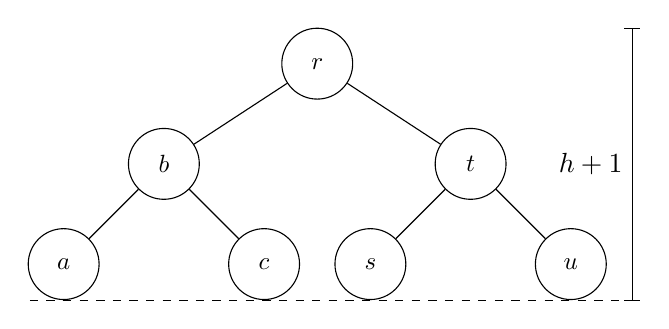
\begin{tikzpicture}[baseline={(0,0)},node distance={20mm},main/.style={draw, circle, scale=0.9, minimum size=10mm}]
    \node[main] (1) [] {$r$};

    \node[main] (0) [below right of=1, xshift=7.5mm] {$t$};
    \node[main] (2) [below right of=0] {$u$};

    \node[main] (3) [below left of=1, xshift=-7.5mm] {$b$};
    \node[main] (4) [below left of=0] {$s$};

    \node[main] (5) [below left of=3] {$a$};
    \node[main] (6) [below right of=3] {$c$};

    \draw (0) -- (1);
    \draw (0) -- (2);
    \draw (1) -- (3);
    \draw (0) -- (4);
    \draw (3) -- (5);
    \draw (3) -- (6);

    \draw (4,0.45) -- (4,-3) node[midway, left] {$h+1$};
    \draw (3.9,0.45) -- (4.1,0.45);
    \draw [dashed] (-3.65,-3.01) -- (3.9,-3.01);
    \draw (3.9,-3.01) -- (4.1,-3.01);
\end{tikzpicture} &
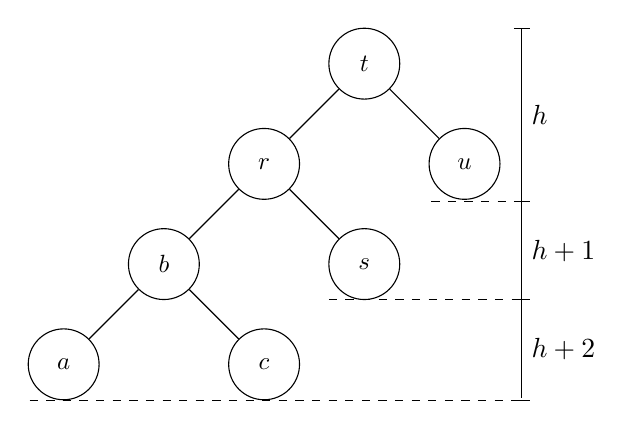
\begin{tikzpicture}[baseline={(0,0)},node distance={20mm},main/.style={draw, circle, scale=0.9, minimum size=10mm}]
    \node[main] (0) {$t$};

    \node[main] (1) [below left of=0] {$r$};
    \node[main] (2) [below right of=0] {$u$};

    \node[main] (3) [below left of=1] {$b$};
    \node[main] (4) [below right of=1] {$s$};

    \node[main] (5) [below left of=3] {$a$};
    \node[main] (6) [below right of=3] {$c$};

    \draw (0) -- (1);
    \draw (0) -- (2);
    \draw (1) -- (3);
    \draw (1) -- (4);
    \draw (3) -- (5);
    \draw (3) -- (6);

    \draw (2,0.45) -- (2,-1.75) node[midway, right] {$h$};
    \draw (1.9,0.45) -- (2.1,0.45);
    \draw [dashed] (0.85,-1.75) -- (1.9,-1.75);
    \draw (1.9,-1.75) -- (2.1,-1.75);
    \draw (2,-1.75) -- (2,-3) node[midway, right] {$h+1$};
    \draw [dashed] (-0.45,-3) -- (1.9,-3);
    \draw (1.9,-3) -- (2.1,-3);
    \draw (2,-3) -- (2,-4.25) node[midway, right] {$h+2$};
    \draw [dashed] (-4.25,-4.275) -- (1.9,-4.275);
    \draw (1.9,-4.275) -- (2.1, -4.275);
\end{tikzpicture}
\end{tabular}
\caption{Esempio di \emph{rotazione verso sinistra} del \emph{nodo} $t$}
\end{figure}\noindent
Da questo esempio si vede anche che applicando una rotazione su un \emph{nodo}
e applicando poi la rotazione inversa sullo stesso \emph{nodo}, si riottiene
l'\emph{albero} di partenza della prima rotazione.

\subsection{Inserimento}
A questo punto, possiamo affrontare l'argomento \emph{inserimento}, che nei
principi generali non si discosta molto da quanto visto per gli \emph{alberi
binari di ricerca}. In particolare, la posizione di inserimento viene
ricercata con le stesse regole, ma in più il nuovo \emph{nodo} viene \q{colorato}
di rosso.

\noindent
Ovviamente, come già accennato, l'inserimento di un \emph{nodo} può comportare
la violazione dei \emph{vincoli di bilanciamento}. È quindi opportuno che ad
ogni inserimento, se necessario, l'\emph{albero} venga ribilanciato.

\begin{minicode}{Implementazione insertNode per Alberi Red-Black}
\ind\bc{TREE} insertNode(\bc{TREE} t, \bc{ITEM} k, \bc{ITEM} v)\\
    \bc{TREE} p = nil\hfill\com{Riferimento al \emph{padre}}
    \bc{TREE} u = t\\
    \indf while (u $\neq$ nil and u.key $\neq$ k) do\hfill\com{Cerca la posizione di inserimento}
        p = u\\
        u = iif(k < u.key, u.left, u.right)\\
    \indf if (u $\neq$ nil and u.key == k) then\hfill\com{Chiave già presente}
        u.value = v\\
    \indf else\\
        \bc{TREE} newTree = Tree(k, v)\hfill\com{Crea un nuovo \emph{nodo}}
        link(p, newTree, k)\hfill\com{Inserisce il nuovo \emph{nodo}}
        balanceInsert(newTree)\hfill\com{Garantisce il bilanciamento dell'\emph{albero}}
        \indff if (p == nil) then\hfill\com{Il \emph{nodo} creato è il primo dell'\emph{albero}}
            t = newTree\\
    \indf return t
\end{minicode}\noindent
La funzione \texttt{balanceInsert} si occupa di garantire il rispetto di tutti i
\emph{vincoli di bilanciamento} modificando la colorazione dei \emph{nodi} o
applicando delle rotazioni.

Questa funzione procede con un approccio bottom-up a partire dal \emph{nodo}
inserito. A mano a mano che risale, i \emph{figli} di ogni \emph{nodo} rosso
vengono colorati di nero, garantendo così il rispetto del \emph{vincolo 3}.
Tutte le violazioni ancora irrisolte vengono in questo modo spostate verso
l'alto. Quando infine viene raggiunta la \emph{radice}, questa viene colorata
di nero come richiesto dal \emph{vincolo 1}, ma ciò si rende necessario solo se
il \emph{nodo} inserito era proprio la \emph{radice} o se risalendo
l'\emph{albero} era stata colorata di rosso.

\begin{note}
    Le operazioni di ripristino sono necessarie solo quando due \emph{nodi}
    consecutivi sono rossi.
\end{note}
\begin{note}
    Ogni \emph{nodo} inserito viene in automatico colorato di rosso perché in
    questo modo c'è la possibilità che non sia necessario ribilanciare
    l'\emph{albero}. Al contrario, l'inserimento di un \emph{nodo} nero
    comporta sempre un ribilanciamento perché viene modificata
    l'\emph{altezza nera} dell'\emph{albero}.
\end{note}

\medskip\noindent
\begin{minipage}[c]{0.6\textwidth}
Quando si inserisce un \emph{nodo}, per capire se i \emph{vincoli di bilanciamento}
sono stati violati, è sufficiente analizzare quattro \emph{nodi}:
\begin{itemize}
    \item Il \emph{nodo} $t$ appena inserito;
    \item Il \emph{padre} $p$ di $t$;
    \item Il \emph{padre} $n$ di $p$ o, equivalentemente, il \emph{nonno} di $t$;
    \item Il secondo \emph{figlio} $z$ di $n$, ovvero il \emph{fratello} di $p$ o
    lo \emph{zio} di $t$;
\end{itemize}
\end{minipage}
\hfill
\begin{minipage}[c]{0.38\textwidth}
\begin{center}
\begin{tikzpicture}[node distance={20mm},main/.style={draw, circle, scale=1, minimum size=10mm}]
    \node[main] (0) {$n$};
    \node[main] (1) [below left of=0] {$p$};
    \node[main] (2) [below right of=0] {$z$};
    \node[main] (3) [below left of=1] {$t$};

    \draw (0) -- (1);
    \draw (0) -- (2);
    \draw (1) -- (3);
\end{tikzpicture}
\end{center}
\end{minipage}

\medskip\noindent
A seconda del colore di questi quattro \emph{nodi} si configurano 7 possibili
casi.

\paragraph{Caso 1 - Il nuovo nodo non ha padre}
Questo caso si configura quando viene inserita la \emph{radice} dell'\emph{albero}
o quando risalendo si è arrivati alla \emph{radice}. A questo punto l'unico
vincolo che potrebbe risultare violato è il numero 1, quindi è sufficiente
colorare il \emph{nodo} di nero.

\begin{figure}[ht]
    \centering
    \begin{graph}
        \tikzset{rb/.style={main, font=\large\boldmath}}
        \tikzset{b/.style={rb, fill=black, color=black, text=red}}
        \tikzset{r/.style={rb, fill=red, color=red, text=black}}
        \tikzset{nil/.style={rectangle, fill=black, color=black, text=red, font=\ttfamily\large}}
    
        \node[r] (0) {$t$};
        \node[main] (1) [below left of=0] {};
        \node[main] (2) [below right of=0] {};
        \node[] (l1) [left of=0] {$(1)$};
        \node[] (l2) [right of=0, xshift=20] {\Huge$\Longrightarrow$};
    
        \node[b] (3) [right of=l2, xshift=20] {$t$};
        \node[] (l3) [right of=3] {$t=\texttt{nil}$};
        \node[main] (4) [below left of=3] {};
        \node[main] (5) [below right of=3] {};
    
        \node[inner sep=0] (6) [below left of=1, xshift=15, yshift=-20] {};
        \node[inner sep=0] (7) [below right of=1, xshift=-15, yshift=-20] {};
        \node[inner sep=0] (8) [below left of=2, xshift=15, yshift=-20] {};
        \node[inner sep=0] (9) [below right of=2, xshift=-15, yshift=-20] {};
    
        \node[inner sep=0] (10) [below left of=4, xshift=15, yshift=-20] {};
        \node[inner sep=0] (11) [below right of=4, xshift=-15, yshift=-20] {};
        \node[inner sep=0] (12) [below left of=5, xshift=15, yshift=-20] {};
        \node[inner sep=0] (13) [below right of=5, xshift=-15, yshift=-20] {};
    
        \path[-]  (0)   edge (1)
                  (0)   edge (2)
                  (3)   edge (4)
                  (3)   edge (5)
                  (1)   edge (6)
                  (1)   edge (7)
                  (2)   edge (8)
                  (2)   edge (9)
                  (4)   edge (10)
                  (4)   edge (11)
                  (5)   edge (12)
                  (5)   edge (13)
                  (6)   edge node[midway, above, yshift=10] {$A$} (7)
                  (8)   edge node[midway, above, yshift=10] {$B$} (9)
                  (10)  edge node[midway, above, yshift=10] {$A$} (11)
                  (12)  edge node[midway, above, yshift=10] {$B$} (13);
      \end{graph}
    \caption{Risoluzione del caso 1}
\end{figure}

\paragraph{Caso 2 - Il padre di \bm{$t$} è nero}
In questo caso non serve fare nulla, poiché nessun vincolo può risultare violato.

\begin{figure}[h!]
    \centering
    \begin{graph}
        \tikzset{rb/.style={main, font=\large\boldmath}}
        \tikzset{b/.style={rb, fill=black, color=black, text=red}}
        \tikzset{r/.style={rb, fill=red, color=red, text=black}}
        \tikzset{nil/.style={rectangle, fill=black, color=black, text=red, font=\ttfamily\large}}
    
        \node[r] (0) {$t$};
        \node[b] (1) [below left of=0] {};
        \node[b] (2) [below right of=0] {};
        \node[] (l1) [left of=0] {$(2)$};
    
        \node[b] (3) [above right of=0, xshift=20] {$p$};
        \node[main] (4) [below right of=3, xshift=20] {};
        \node[] (l2) [right of=3, xshift=40] {$t=\texttt{nil}$};
        \node[] (l3) [right of=4, xshift=-20] {$(Ok)$};
    
        \node[inner sep=0] (6) [below left of=1, xshift=15, yshift=-20] {};
        \node[inner sep=0] (7) [below right of=1, xshift=-15, yshift=-20] {};
        \node[inner sep=0] (8) [below left of=2, xshift=15, yshift=-20] {};
        \node[inner sep=0] (9) [below right of=2, xshift=-15, yshift=-20] {};
    
        \node[inner sep=0] (10) [below left of=4, xshift=15, yshift=-20] {};
        \node[inner sep=0] (11) [below right of=4, xshift=-15, yshift=-20] {};
    
        \path[-]  (0)   edge (1)
                  (0)   edge (2)
                  (0)   edge (3)
                  (3)   edge (4)
                  (1)   edge (6)
                  (1)   edge (7)
                  (2)   edge (8)
                  (2)   edge (9)
                  (4)   edge (10)
                  (4)   edge (11)
                  (6)   edge node[midway, above, yshift=10] {$A$} (7)
                  (8)   edge node[midway, above, yshift=10] {$B$} (9)
                  (10)  edge node[midway, above, yshift=10] {$C$} (11);
    \end{graph}
    \caption{Risoluzione del caso 2}
\end{figure}

\paragraph{Caso 3 - Sia \bm{$t$} che il padre e lo zio sono rossi}
Poiché $z$ è rosso, è possibile colorare di nero $p$ e $z$ e poi colorare di
rosso $n$. A questo punto, poiché tutti i cammini che passano per $p$ e $z$
passano anche per $n$, l'\emph{altezza nera} certamente non avrà subito variazioni.

A questo punto, è ancora possibile che $n$ violi i \emph{vincoli 1} e \emph{3}.
Di conseguenza, risaliamo l'\emph{albero} ponendo $t=n$ e ripetiamo il ciclo.

\begin{figure}[h!]
    \centering
    \resizebox*{\textwidth}{!}{
    \begin{graph}
        \tikzset{rb/.style={main, font=\large\boldmath}}
        \tikzset{b/.style={rb, fill=black, color=black, text=red}}
        \tikzset{r/.style={rb, fill=red, color=red, text=black}}
        \tikzset{nil/.style={rectangle, fill=black, color=black, text=red, font=\ttfamily\large}}

        \node[r] (0) {$t$};
        \node[b] (1) [below left of=0, xshift=10] {};
        \node[b] (2) [below right of=0, xshift=-10] {};
        \node[] (l1) [left of=0] {$(3)$};

        \node[r] (3) [above right of=0, xshift=0] {$p$};
        \node[b] (4) [below right of=3, xshift=0] {};

        \node[b] (5) [above right of=3, xshift=30] {$n$};

        \node[inner sep=0] (6) [below left of=1, xshift=15, yshift=-20] {};
        \node[inner sep=0] (7) [below right of=1, xshift=-15, yshift=-20] {};
        \node[inner sep=0] (8) [below left of=2, xshift=15, yshift=-20] {};
        \node[inner sep=0] (9) [below right of=2, xshift=-15, yshift=-20] {};

        \node[inner sep=0] (10) [below left of=4, xshift=15, yshift=-20] {};
        \node[inner sep=0] (11) [below right of=4, xshift=-15, yshift=-20] {};

        \node[r] (12) [below right of=5, xshift=30] {$z$};
        \node[b] (13) [below left of=12, xshift=0] {};
        \node[b] (14) [below right of=12, xshift=0] {};

        \node[inner sep=0] (15) [below left of=13, xshift=15, yshift=-20] {};
        \node[inner sep=0] (16) [below right of=13, xshift=-15, yshift=-20] {};
        \node[inner sep=0] (17) [below left of=14, xshift=15, yshift=-20] {};
        \node[inner sep=0] (18) [below right of=14, xshift=-15, yshift=-20] {};

        \path[-]  (0)   edge (1)
                (0)   edge (2)
                (0)   edge (3)
                (3)   edge (4)
                (3)   edge (5)
                (1)   edge (6)
                (1)   edge (7)
                (2)   edge (8)
                (2)   edge (9)
                (4)   edge (10)
                (4)   edge (11)
                (5)   edge (12)
                (12)  edge (13)
                (12)  edge (14)
                (13)  edge (15)
                (13)  edge (16)
                (14)  edge (17)
                (14)  edge (18)
                (6)   edge node[midway, above, yshift=10] {$A$} (7)
                (8)   edge node[midway, above, yshift=10] {$B$} (9)
                (10)  edge node[midway, above, yshift=10] {$C$} (11)
                (15)  edge node[midway, above, yshift=10] {$D$} (16)
                (17)  edge node[midway, above, yshift=10] {$E$} (18);
        
        \node[] (l2) [right of=12, xshift=30] {\Huge$\Longrightarrow$};

        \node[b] (23) [right of=l2, xshift=30] {$p$};
        \node[b] (24) [below right of=23, xshift=0] {};

        \node[r] (20) [below left of=23] {$t$};
        \node[b] (21) [below left of=20, xshift=10] {};
        \node[b] (22) [below right of=20, xshift=-10] {};

        \node[r] (25) [above right of=23, xshift=30] {$n$};

        \node[inner sep=0] (26) [below left of=21, xshift=15, yshift=-20] {};
        \node[inner sep=0] (27) [below right of=21, xshift=-15, yshift=-20] {};
        \node[inner sep=0] (28) [below left of=22, xshift=15, yshift=-20] {};
        \node[inner sep=0] (29) [below right of=22, xshift=-15, yshift=-20] {};

        \node[inner sep=0] (30) [below left of=24, xshift=15, yshift=-20] {};
        \node[inner sep=0] (31) [below right of=24, xshift=-15, yshift=-20] {};

        \node[b] (32) [below right of=25, xshift=30] {$z$};
        \node[b] (33) [below left of=32, xshift=0] {};
        \node[b] (34) [below right of=32, xshift=0] {};

        \node[inner sep=0] (35) [below left of=33, xshift=15, yshift=-20] {};
        \node[inner sep=0] (36) [below right of=33, xshift=-15, yshift=-20] {};
        \node[inner sep=0] (37) [below left of=34, xshift=15, yshift=-20] {};
        \node[inner sep=0] (38) [below right of=34, xshift=-15, yshift=-20] {};

        \node[] (l3) [right of=25, xshift=40] {$t=n$};

        \path[-]  (20)  edge (21)
                (20)  edge (22)
                (20)  edge (23)
                (23)  edge (24)
                (23)  edge (25)
                (21)  edge (26)
                (21)  edge (27)
                (22)  edge (28)
                (22)  edge (29)
                (24)  edge (30)
                (24)  edge (31)
                (25)  edge (32)
                (32)  edge (33)
                (32)  edge (34)
                (33)  edge (35)
                (33)  edge (36)
                (34)  edge (37)
                (34)  edge (38)
                (26)  edge node[midway, above, yshift=10] {$A$} (27)
                (28)  edge node[midway, above, yshift=10] {$B$} (29)
                (30)  edge node[midway, above, yshift=10] {$C$} (31)
                (35)  edge node[midway, above, yshift=10] {$D$} (36)
                (37)  edge node[midway, above, yshift=10] {$E$} (38);
    \end{graph}}
    \caption{Risoluzione del caso 3}
\end{figure}

\newpage
\paragraph{Caso 4 - Sia \bm{$t$} che il padre sono rossi e lo zio è nero}
\begin{enumerate}[label=\alph*.]
    \item \emph{$t$ è il figlio destro di $p$ e $p$ è il figlio sinistro di $n$}:
    viene eseguita una rotazione verso sinistra partendo dal \emph{nodo} $p$ in
    modo da rendere $p$ il \emph{figlio sinistro} di $t$ e potersi così ricondurre
    al \emph{caso 5a}. In questo caso vengono coinvolti soltanto i \emph{nodi}
    $p$ e $t$ che essendo entrambi rossi, non influenzano l'\emph{altezza nera};
    \item \emph{$t$ è il figlio sinistro di $p$ e $p$ è il figlio destro di $n$}:
    viene eseguita una rotazione verso destra partendo dal \emph{nodo} $p$ in
    modo da rendere $p$ il \emph{figlio destro} di $t$ e potersi così ricondurre
    al \emph{caso 5b}. In questo caso vengono coinvolti soltanto i \emph{nodi}
    $p$ e $t$ che essendo entrambi rossi, non influenzano l'\emph{altezza nera};
\end{enumerate}

\begin{figure}[h!]
    \centering
    \resizebox*{\textwidth}{!}{
    \begin{graph}
        \tikzset{rb/.style={main, font=\large\boldmath}}
        \tikzset{b/.style={rb, fill=black, color=black, text=red}}
        \tikzset{r/.style={rb, fill=red, color=red, text=black}}
        \tikzset{nil/.style={rectangle, fill=black, color=black, text=red, font=\ttfamily\large}}

        \node[r] (0) {$t$};
        \node[b] (1) [below left of=0, xshift=10] {};
        \node[b] (2) [below right of=0, xshift=-10] {};

        \node[r] (3) [above left of=0, xshift=0] {$p$};
        \node[b] (4) [below left of=3, xshift=0] {};

        \node[b] (5) [above right of=3, xshift=40] {$n$};
        \node[] (l1) [left of=5, xshift=-10] {$\begin{array}{l}
        (4a)\\
        (4b)\text{ speculare}
        \end{array}$};

        \node[inner sep=0] (6) [below left of=1, xshift=15, yshift=-20] {};
        \node[inner sep=0] (7) [below right of=1, xshift=-15, yshift=-20] {};
        \node[inner sep=0] (8) [below left of=2, xshift=15, yshift=-20] {};
        \node[inner sep=0] (9) [below right of=2, xshift=-15, yshift=-20] {};

        \node[inner sep=0] (10) [below left of=4, xshift=15, yshift=-20] {};
        \node[inner sep=0] (11) [below right of=4, xshift=-15, yshift=-20] {};

        \node[b] (12) [below right of=5, xshift=40] {$z$};
        \node[main] (13) [below left of=12, xshift=0] {};
        \node[main] (14) [below right of=12, xshift=0] {};

        \node[inner sep=0] (15) [below left of=13, xshift=15, yshift=-20] {};
        \node[inner sep=0] (16) [below right of=13, xshift=-15, yshift=-20] {};
        \node[inner sep=0] (17) [below left of=14, xshift=15, yshift=-20] {};
        \node[inner sep=0] (18) [below right of=14, xshift=-15, yshift=-20] {};

        \path[-]  (0)   edge (1)
                (0)   edge (2)
                (0)   edge (3)
                (3)   edge (4)
                (3)   edge (5)
                (1)   edge (6)
                (1)   edge (7)
                (2)   edge (8)
                (2)   edge (9)
                (4)   edge (10)
                (4)   edge (11)
                (5)   edge (12)
                (12)  edge (13)
                (12)  edge (14)
                (13)  edge (15)
                (13)  edge (16)
                (14)  edge (17)
                (14)  edge (18)
                (6)   edge node[midway, above, yshift=10] {$B$} (7)
                (8)   edge node[midway, above, yshift=10] {$C$} (9)
                (10)  edge node[midway, above, yshift=10] {$A$} (11)
                (15)  edge node[midway, above, yshift=10] {$D$} (16)
                (17)  edge node[midway, above, yshift=10] {$E$} (18);
        
        \node[] (l2) [right of=12, xshift=40] {\Huge$\Longrightarrow$};

        \node[r] (23) [right of=l2, xshift=40] {$t$};
        \node[b] (24) [below right of=23, xshift=0] {};

        \node[r] (20) [below left of=23] {$p$};
        \node[b] (21) [below left of=20, xshift=10] {};
        \node[b] (22) [below right of=20, xshift=-10] {};

        \node[b] (25) [above right of=23, xshift=30] {$n$};

        \node[inner sep=0] (26) [below left of=21, xshift=15, yshift=-20] {};
        \node[inner sep=0] (27) [below right of=21, xshift=-15, yshift=-20] {};
        \node[inner sep=0] (28) [below left of=22, xshift=15, yshift=-20] {};
        \node[inner sep=0] (29) [below right of=22, xshift=-15, yshift=-20] {};

        \node[inner sep=0] (30) [below left of=24, xshift=15, yshift=-20] {};
        \node[inner sep=0] (31) [below right of=24, xshift=-15, yshift=-20] {};

        \node[b] (32) [below right of=25, xshift=30] {$z$};
        \node[main] (33) [below left of=32, xshift=0] {};
        \node[main] (34) [below right of=32, xshift=0] {};

        \node[inner sep=0] (35) [below left of=33, xshift=15, yshift=-20] {};
        \node[inner sep=0] (36) [below right of=33, xshift=-15, yshift=-20] {};
        \node[inner sep=0] (37) [below left of=34, xshift=15, yshift=-20] {};
        \node[inner sep=0] (38) [below right of=34, xshift=-15, yshift=-20] {};

        \node[] (l3) [right of=25, xshift=40] {$t=p$};

        \path[-]  (20)  edge (21)
                (20)  edge (22)
                (20)  edge (23)
                (23)  edge (24)
                (23)  edge (25)
                (21)  edge (26)
                (21)  edge (27)
                (22)  edge (28)
                (22)  edge (29)
                (24)  edge (30)
                (24)  edge (31)
                (25)  edge (32)
                (32)  edge (33)
                (32)  edge (34)
                (33)  edge (35)
                (33)  edge (36)
                (34)  edge (37)
                (34)  edge (38)
                (26)  edge node[midway, above, yshift=10] {$A$} (27)
                (28)  edge node[midway, above, yshift=10] {$B$} (29)
                (30)  edge node[midway, above, yshift=10] {$C$} (31)
                (35)  edge node[midway, above, yshift=10] {$D$} (36)
                (37)  edge node[midway, above, yshift=10] {$E$} (38);
    \end{graph}}
    \caption{Risoluzione del caso 4}
\end{figure}

\paragraph{Caso 5 - Sia \bm{$t$} che il padre sono rossi e lo zio è nero}
\begin{enumerate}[label=\alph*.]
    \item \emph{$t$ è il figlio sinistro di $p$ e $p$ è il figlio sinistro di $n$}:
    viene eseguita una rotazione verso destra partendo dal \emph{nodo} $n$ in modo
    da rendere $t$ ed $n$ \emph{figli} di $p$. Quindi, colorando di rosso $n$
    e di nero $p$ ci si porta in una situazione nella quale tutti i
    \emph{vincoli di bilanciamento} sono rispettati e l'\emph{altezza nera} è
    uguale alla situazione iniziale;
    \item \emph{$t$ è il figlio destro di $p$ e $p$ è il figlio destro di $n$}:
    viene eseguita una rotazione verso sinistra partendo dal \emph{nodo} $n$ in
    modo da rendere $t$ ed $n$ \emph{figli} di $p$. Quindi, colorando di rosso
    $n$ e di nero $p$ ci si porta in una situazione nella quale tutti i
    \emph{vincoli di bilanciamento} sono rispettati e l'\emph{altezza nera} è
    uguale alla situazione iniziale;
\end{enumerate}

\begin{figure}[h!]
    \centering
    \resizebox*{0.95\textwidth}{!}{
    \begin{graph}
        \tikzset{rb/.style={main, font=\large\boldmath}}
        \tikzset{b/.style={rb, fill=black, color=black, text=red}}
        \tikzset{r/.style={rb, fill=red, color=red, text=black}}
        \tikzset{nil/.style={rectangle, fill=black, color=black, text=red, font=\ttfamily\large}}

        \node[r] (0) {$t$};
        \node[b] (1) [below left of=0, xshift=10] {};
        \node[b] (2) [below right of=0, xshift=-10] {};

        \node[r] (3) [above right of=0, xshift=0] {$p$};
        \node[b] (4) [below right of=3, xshift=0] {};

        \node[b] (5) [above right of=3, xshift=40] {$n$};
        \node[] (l1) [left of=5, xshift=-10] {$\begin{array}{l}
        (5a)\\
        (5b)\text{ speculare}
        \end{array}$};

        \node[inner sep=0] (6) [below left of=1, xshift=15, yshift=-20] {};
        \node[inner sep=0] (7) [below right of=1, xshift=-15, yshift=-20] {};
        \node[inner sep=0] (8) [below left of=2, xshift=15, yshift=-20] {};
        \node[inner sep=0] (9) [below right of=2, xshift=-15, yshift=-20] {};

        \node[inner sep=0] (10) [below left of=4, xshift=15, yshift=-20] {};
        \node[inner sep=0] (11) [below right of=4, xshift=-15, yshift=-20] {};

        \node[b] (12) [below right of=5, xshift=40] {$z$};
        \node[main] (13) [below left of=12, xshift=0] {};
        \node[main] (14) [below right of=12, xshift=0] {};

        \node[inner sep=0] (15) [below left of=13, xshift=15, yshift=-20] {};
        \node[inner sep=0] (16) [below right of=13, xshift=-15, yshift=-20] {};
        \node[inner sep=0] (17) [below left of=14, xshift=15, yshift=-20] {};
        \node[inner sep=0] (18) [below right of=14, xshift=-15, yshift=-20] {};

        \path[-]  (0)   edge (1)
                (0)   edge (2)
                (0)   edge (3)
                (3)   edge (4)
                (3)   edge (5)
                (1)   edge (6)
                (1)   edge (7)
                (2)   edge (8)
                (2)   edge (9)
                (4)   edge (10)
                (4)   edge (11)
                (5)   edge (12)
                (12)  edge (13)
                (12)  edge (14)
                (13)  edge (15)
                (13)  edge (16)
                (14)  edge (17)
                (14)  edge (18)
                (6)   edge node[midway, above, yshift=10] {$B$} (7)
                (8)   edge node[midway, above, yshift=10] {$C$} (9)
                (10)  edge node[midway, above, yshift=10] {$A$} (11)
                (15)  edge node[midway, above, yshift=10] {$D$} (16)
                (17)  edge node[midway, above, yshift=10] {$E$} (18);
        
        \node[] (l2) [right of=12, xshift=40] {\Huge$\Longrightarrow$};

        \node[r] (23) [right of=l2, xshift=40] {$t$};
        \node[b] (24) [below right of=23, xshift=0] {};

        \node[b] (20) [below left of=23] {};

        \node[b] (25) [above right of=23, xshift=30] {$p$};

        \node[inner sep=0] (26) [below left of=20, xshift=15, yshift=-20] {};
        \node[inner sep=0] (27) [below right of=20, xshift=-15, yshift=-20] {};
        \node[inner sep=0] (28) [below left of=22, xshift=15, yshift=-20] {};
        \node[inner sep=0] (29) [below right of=22, xshift=-15, yshift=-20] {};

        \node[inner sep=0] (30) [below left of=24, xshift=15, yshift=-20] {};
        \node[inner sep=0] (31) [below right of=24, xshift=-15, yshift=-20] {};

        \node[r] (32) [below right of=25, xshift=30] {$n$};
        \node[b] (33) [below left of=32, xshift=0] {};
        \node[b] (34) [below right of=32, xshift=0] {$z$};

        \node[inner sep=0] (35) [below left of=33, xshift=15, yshift=-20] {};
        \node[inner sep=0] (36) [below right of=33, xshift=-15, yshift=-20] {};
        \node[main] (37) [below left of=34, xshift=10, yshift=-20] {};
        \node[main] (38) [below right of=34, xshift=-10, yshift=-20] {};

        \node[inner sep=0] (39) [below left of=37, xshift=15, yshift=-20] {};
        \node[inner sep=0] (40) [below right of=37, xshift=-15, yshift=-20] {};
        \node[inner sep=0] (41) [below left of=38, xshift=15, yshift=-20] {};
        \node[inner sep=0] (42) [below right of=38, xshift=-15, yshift=-20] {};

        \node[] (l3) [right of=25, xshift=40] {$t=\texttt{nil}$};

        \path[-]  (20)  edge (26)
                (20)  edge (27)
                (20)  edge (23)
                (23)  edge (24)
                (23)  edge (25)
                (24)  edge (30)
                (24)  edge (31)
                (25)  edge (32)
                (32)  edge (33)
                (32)  edge (34)
                (33)  edge (35)
                (33)  edge (36)
                (34)  edge (37)
                (34)  edge (38)
                (37)  edge (39)
                (37)  edge (40)
                (38)  edge (41)
                (38)  edge (42)
                (26)  edge node[midway, above, yshift=10] {$A$} (27)
                (30)  edge node[midway, above, yshift=10] {$B$} (31)
                (35)  edge node[midway, above, yshift=10] {$C$} (36)
                (39)  edge node[midway, above, yshift=10] {$D$} (40)
                (41)  edge node[midway, above, yshift=10] {$E$} (42);
    \end{graph}}
    \caption{Risoluzione del caso 5}
\end{figure}

\begin{minicode}{Implementazione balanceInsert}
\ind balanceInsert(\bc{TREE} t)\\
    t.color = RED\hfill\com{Il \emph{nodo} inserito viene inizialmente colorato di rosso}
    \indf while (t $\neq$ nil) do\\
        \bc{TREE} p = t.parent\hfill\com{\emph{Padre}}
        \bc{TREE} n = iif(p $\neq$ nil, p.parent, nil)\hfill\com{\emph{Nonno}}
        \bc{TREE} z = iif(n $\neq$ nil, iif(n.left == p, n.right, n.left), nil)\hfill\com{\emph{Zio}}
        \indff if (p == nil) then\hfill\com{Caso 1}
            t.color = BLACK\\
            t = nil\\
        \indff else if (p.color == BLACK) then\hfill\com{Caso 2}
            t = nil\\
        \indff else if (z.color == RED) then\hfill\com{Caso 3}
            p.color = BLACK\\
            z.color = BLACK\\
            n.color = RED\\
            t = n\\
        \indff else\\
            \indfff if (t == p.right and p == n.left) then\hfill\com{Caso 4a}
                rotateLeft(p)\\
                t = p\\
            \indfff else if (t == p.left and p == n.right) then\hfill\com{Caso 4b}
                rotateRight(p)\\
                t = p\\
            \indfff else\\
                \indffff if (t == p.left and p == n.left) then\hfill\com{Caso 5a}
                    rotateRight(n)\\
                \indffff else if (t == p.right and p == n.right) then\hfill\com{Caso 5b}
                    rotateLeft(n)\\
            \indfff\\
                p.color = BLACK\\
                n.color = RED\\
                t = nil
\end{minicode}

\paragraph{Complessità della balanceInsert}
Non è difficile rendersi conto che tutte le istruzione interne al ciclo
\texttt{while} hanno \emph{complessità} $O(1)$. Di conseguenza, la
\emph{complessità} totale della funzione dipende dal numero di volte che viene
eseguito il ciclo. Poiché $t$ quando viene inserito è una \emph{foglia},\footnotemark
il caso peggiore è quello in cui il ribilanciamento coinvolge tutti i \emph{livelli}
e quindi termina solo dopo aver raggiunto la \emph{radice}.
\footnotetext{I \emph{nodi} di un \emph{albero} vengono sempre inseriti al
\emph{livello} delle \emph{foglie}}

In quel caso la \emph{complessità} dipende dall'\emph{altezza} dell'\emph{albero}.
Vedremo che negli \emph{Alberi Red-Black} esiste una relazione ben precisa tra
la loro \emph{altezza} il numero di noi \emph{nodi} che contengono.
\newpage
\subsection{Altezza degli Alberi Red-Black}
\begin{definition}[Numero massimo di nodi interni]
    In un Albero Red-Black, un sottoalbero di radice $u$ contiene un numero
    $n\geq 2^{bh(u)}-1$ di nodi interni.
\end{definition}
\begin{proof}[Dimostrazione]
    Procediamo per induzione sull'altezza del nodo $u$.
    \paragraph{Caso base} Dimostro la disequazione per $h=0$:

    se $h=0$, $u$ è una \emph{foglia} \texttt{Nil} e quindi il \emph{sottoalbero}
    con \emph{radice} $u$ non può contenere \emph{nodi interni}, quindi $n$ deve
    per forza valere $0$. Poiché:
    \[n\geq2^{bh(u)}-1=2^0-1=1-1=0\]
    ciò è confermato e quindi il caso base risulta verificato.

    \paragraph{Passo induttivo} Ipotizzo che $n\geq2^{bh(u)}-1$ per ogni
    \emph{albero} con \emph{radice} $u$ e \emph{altezza} $h\leq1$. Dimostro la
    disequazione per $h>1$:

    se $h>1$, $u$ è certamente un \emph{nodo interno} e quindi ha due \emph{figli}.
    Ogni \emph{figlio} di $u$ ha un \emph{altezza nera} che è pari a $bh(u)$ se
    è rosso e $bh(u)-1$ se è nero. Ogni \emph{sottoalbero} con \emph{radice} uno
    dei \emph{figli} di $u$ ha \emph{altezza} $h-1$ e quindi, per ipotesi induttiva,
    so che ognuno di quei sottoalberi ha almeno $2^{bh(u)-1}-1$ \emph{nodi interni}.

    Allora, per il \emph{sottoalbero} con \emph{radice} $u$ vale:
    \[n\geq2\cdot\left(2^{bh(u)-1}-1\right)+1\]
    cioè, il numero di \emph{nodi interni} del \emph{sottoalbero} con \emph{radice}
    $u$ è pari, almeno, alla somma dei limiti inferiori al numero di \emph{nodi
    interni} dei \emph{sottoalberi} che hanno come \emph{radice} un \emph{figlio}
    di $u$, più $1$, perché bisogna contare anche il \emph{nodo} $u$ stesso.

    Poiché vale seguente catena di uguaglianze:
    \[n\geq2\cdot\left(2^{bh(u)-1}-1\right)+1=2\cdot\left(\frac{2^{bh(u)}}{2}-1
    \right)+1=2^{bh(u)}-2+1=2^{bh(u)}-1\]
    il passo induttivo risulta verificato.
\end{proof}

\begin{definition}[Quota nera minima]
    In un Albero Red-Black, almeno la metà dei nodi dalla radice a una foglia
    deve essere nera.
\end{definition}
\begin{proof}[Dimostrazione]
    Per il secondo \emph{vincolo di bilanciamento}, i \emph{figli} di un
    \emph{nodo} rosso devono essere neri e, poiché la situazione in cui sono
    presenti il minor numero di \emph{nodi} neri è quando \emph{nodi} rossi
    e neri sono alternati, almeno la metà dei \emph{nodi} devono essere neri.
\end{proof}

\begin{definition}[Lunghezza massima dei cammini semplici]
    In un \emph{Albero Red-Black}, dati due \emph{cammini semplici}, dalla
    \emph{radice} a due \emph{foglie}, non è possibile che uno sia lungo più
    del doppio dell'altro.
\end{definition}
\begin{proof}[Dimostrazione]
    Per il quarto \emph{vincolo di bilanciamento}, tutti i \emph{cammini} da
    un \emph{nodo} ad una \emph{foglia} hanno lo stesso numero di \emph{nodi}
    neri e, per la definizione precedente, almeno la metà di quei \emph{nodi}
    deve essere nera. Di conseguenza, il caso più sbilanciato è quello in cui
    un \emph{cammino} è costituito da soli \emph{nodi} neri e l'altro da
    \emph{nodi} neri e rossi alternati e quindi si ha che il secondo \emph{cammino}
    è lungo il doppio del primo.
\end{proof}

\begin{definition}[Altezza massima di un Albero Red-Black]
    L'\emph{altezza} massima di un \emph{Albero Red-Black} con $n$ \emph{nodi
    interni} è al più $2\log(n+1)$.
\end{definition}
\begin{proof}[Dimostrazione]
    Vale quanto segue:
    \[n\geq2^{bh(u)}-1\begin{array}[t]{cll}
        \Leftrightarrow & n\geq2^{h/2}-1 & \quad\hyperref[def:52]{\emph{Quota nera minima}}\\
        \Leftrightarrow & n+1\geq2^{h/2}\\
        \Leftrightarrow & \log(n+1)\geq h^2 & \quad\emph{Applicazione logaritmo ai termini}\\
        \Leftrightarrow & h\leq2\log(n+1)
    \end{array}\]
\end{proof}

\paragraph{Complessità funzione insertNode}
Fatte queste considerazioni sull'\emph{altezza} massima degli \emph{Alberi
Red-Black}, possiamo affermare che la \emph{complessità} della funzione
\texttt{insertNode} è $O(\log n)$. Questo è vero in quanto costa $O(\log n)$
discendere l'\emph{albero} dalla \emph{radice} al punto di inserimento, costa
$O(1)$ inserire il \emph{nodo} e infine, costa $O(\log n)$ ribilanciare
l'\emph{albero} nel caso peggiore, il caso 3.

\subsection{Cancellazione}
Similmente a quanto visto per l'inserimento, la funzione \texttt{removeNode} per
gli \emph{Alberi Red-Black} è costruita a partire dalla controparte per
\emph{alberi binari di ricerca} ed è costituita da un insieme di casistiche che
possono comportare o meno, la necessità di ribilanciare l'\emph{albero}.

Le operazioni di ribilanciamento si rendono necessarie soltanto quando viene
rimosso un \emph{nodo} nero. Ciò è vero in quanto l'eliminazione di un \emph{nodo}
nero comporta sicuramente una variazione dell'\emph{altezza nera} e potrebbe
anche portare ad avere due \emph{nodi} rossi in posizioni consecutive.

Più in generale, quando viene rimosso un \emph{nodo} nero possono essere violati
i \emph{vincoli} 1, 3 o 4. In particolare:
\begin{itemize}
    \item \emph{Violato il vincolo 1}: viene eliminata la \emph{radice} e la
    nuova \emph{radice} è rossa;
    \item \emph{Violato il vincolo 3}: viene eliminato un \emph{nodo} che
    aveva il \emph{padre} e almeno uno dei \emph{figli} rossi;
    \item \emph{Violato il vincolo 4}: ogni volta che viene eliminato un
    \emph{nodo} nero, l'\emph{altezza} nera cambia;
\end{itemize}

\begin{minicode}{Implementazione removeNode per Alberi Red-Black}
\ind\bc{TREE} removeNode(\bc{TREE} t, \bc{ITEM} k)\\
    \bc{TREE} u = lookupNode(t, k)\\
    \indf if (u $\neq$ nil) then\\
        \indff if (u.left == nil and u.right == nil) then\hfill\com{Caso 1}
            link(u.parent, nil, k)\hfill\com{Rimuove il \emph{figlio}}
            delete u\\
        \indff else if (u.left $\neq$ nil and u.right $\neq$ nil) then\hfill\com{Caso 3}
            \bc{TREE} s = successorNode(u)\\
            link(s.parent, s.right, s.key)\hfill\com{Attacca il \emph{figlio} di $s$ al \emph{padre} di $s$}
            u.key = s.key\hfill\com{Copia su $u$ la chiave di $s$}
            u.value = s.value\hfill\com{Copia su $u$ il valore di $s$}
            delete s
\end{minicode}
\begin{codecont}
\begin{minipage}[t]{\textwidth}
        \indff else\hfill\com{Caso 2 con \emph{figlio destro}}
            link(u.parent, u.right, k)\\
            \indfff if (u.parent == nil) then\\
                t = u.right\\
        \\\indff if (u.color == BLACK) then\\
            balanceRemove(t, u)\hfill\com{Garantisce il bilanciamento dell’albero}
    \indf return t
\end{minipage}
\end{codecont}

\begin{minicode}{Implementazione balanceRemove}
\ind balanceRemove(\bc{TREE} r, \bc{TREE} t)\\
    \indf while (t $\neq$ r and t.color == BLACK) do\hfill\com{Il ciclo termina quando $t$ diventa}
    \mbox{}\hfill\com{la \emph{radice} o un \emph{nodo} rosso}
    \bc{TREE} p = t.parent\hfill\com{\emph{Padre}}
    \indff if (t == p.left) then\hfill\com{È sicuramente diverso da \texttt{nil}}
        \bc{TREE} f = p.right\hfill\com{\emph{Fratello}}
        \bc{TREE} ns = f.left\hfill\com{\emph{Nipote sinistro}}
        \bc{TREE} nd = f.right\hfill\com{\emph{Nipote destro}}
        \indfff (f.color == RED) then\hfill\com{Caso 1}
            p.color = RED\\
            f.color = BLACK\\
            rotateLeft(p)\\
        \indfff else\\
            \indffff if (ns.color == BLACK and nd.color == BLACK) then\hfill\com{Caso 2}
                f.color = RED\\
                t = p\\
            \indffff else if (ns.color == RED and nd.color == BLACK) then\hfill\com{Caso 3}
                ns.color = BLACK\\
                f.color = RED\\
                rotateRight(f)\\
            \indffff else if (nd.color == RED) then\hfill\com{Caso 4}
                f.color = p.color\\
                p.color = BLACK\\
                nd.color = BLACK\\
                rotateLeft(p)\\
                t = r\hfill\com{Fa terminare il ciclo}
    \indff else\hfill\com{I casi si ripetono simmetrici ai precedenti}
        \dots
\end{minicode}

\paragraph{Complessità della funzione removeNode}
Come per la \texttt{insertNode} anche in questo caso la \emph{complessità}
totale è $O(\log n)$ in quanto dipende dall'\emph{altezza} dell'\emph{albero}.